\documentclass[a4paper,oneside,14pt]{extreport}

\usepackage[T2A]{fontenc}
\usepackage[utf8]{inputenc}
\usepackage[english,russian]{babel}

\usepackage[left=30mm, right=20mm, top=20mm, bottom=20mm]{geometry}

\usepackage{microtype}
\sloppy

\usepackage{setspace}
\onehalfspacing

\usepackage{indentfirst}
\setlength{\parindent}{12.5mm}

\usepackage{titlesec}
\titleformat{\chapter}{\LARGE\bfseries}{\thechapter}{20pt}{\LARGE\bfseries}
\titlespacing*{\chapter}{\parindent}{*2}{*2}
\titleformat{\section}{\Large\bfseries}{\thesection}{20pt}{\Large\bfseries}

\addto{\captionsrussian}{\renewcommand*{\contentsname}{Содержание}}
\usepackage{natbib}
\renewcommand{\bibsection}{\chapter*{Список использованных источников}}

\usepackage{caption}

\usepackage{wrapfig}
\usepackage{float}

\usepackage{graphicx}
\newcommand{\imgwc}[4]
{
	\begin{figure}[#1]
		\center{\includegraphics[width=#2]{inc/img/#3}}
		\caption{#4}
		\label{img:#3}
	\end{figure}
}
\newcommand{\imghc}[4]
{
	\begin{figure}[#1]
		\center{\includegraphics[height=#2]{inc/img/#3}}
		\caption{#4}
		\label{img:#3}
	\end{figure}
}
\newcommand{\imgsc}[4]
{
	\begin{figure}[#1]
		\center{\includegraphics[scale=#2]{inc/img/#3}}
		\caption{#4}
		\label{img:#3}
	\end{figure}
}

\usepackage{pgfplots}
\pgfplotsset{compat=newest}

\usepackage{listings}
\usepackage{listingsutf8}
\lstset{
	basicstyle=\footnotesize\ttfamily,
	keywordstyle=\color{blue},
	stringstyle=\color{red},
	commentstyle=\color{gray},
	numbers=left,
	numberstyle=\tiny,
	numbersep=5pt,
	frame=false,
	breaklines=true,
	breakatwhitespace=true,
	inputencoding=utf8/koi8-r
}

\lstdefinestyle{c}{
	language=C++,
	backgroundcolor=\color{white},
	basicstyle=\footnotesize\ttfamily,
	keywordstyle=\color{blue},
	stringstyle=\color{red},
	commentstyle=\color{gray},
	directivestyle=\color{orange},
	numbers=left,
	numberstyle=\tiny,
	stepnumber=1,
	numbersep=5pt,
	frame=single,
	tabsize=4,
	captionpos=t,
	breaklines=true,
	breakatwhitespace=true,
	escapeinside={\#*}{*)},
	morecomment=[l][\color{magenta}]{\#},
	columns=fullflexible
}

\newcommand{\code}[1]{\texttt{#1}}

\usepackage{amsmath}
\usepackage{amssymb}

\usepackage[unicode]{hyperref}
\hypersetup{hidelinks}

\makeatletter
\newcommand{\vhrulefill}[1]
{
	\leavevmode\leaders\hrule\@height#1\hfill \kern\z@
}
\makeatother

\begin{document}

\begin{titlepage}
	\centering
	
	\begin{wrapfigure}[7]{l}{0.14\linewidth}
		\vspace{5mm}
		\hspace{-5.8mm}
		
\includegraphics[width=0.93\linewidth]{inc/img/bmstu-logo}
	\end{wrapfigure}
	{\singlespacing \footnotesize \bfseries Министерство науки и высшего образования Российской Федерации\\Федеральное государственное бюджетное образовательное учреждение\\высшего образования\\<<Московский государственный технический университет\\имени Н.~Э.~Баумана\\ (национальный исследовательский университет)>>\\(МГТУ им. Н.~Э.~Баумана)\\}

	\vspace{-2.2mm}
	\vhrulefill{0.9mm}\\
	\vspace{-7mm}
	\vhrulefill{0.2mm}\\
	\vspace{2mm}
	
	{\doublespacing \small \raggedright ФАКУЛЬТЕТ \hspace{25mm} «Информатика и системы управления»\\
	КАФЕДРА \hspace{5mm} «Программное обеспечение ЭВМ и информационные технологии»\\}

	\vspace{30mm}
	
	\textbf{ОТЧЕТ}\\
	По лабораторной работе №1 часть 2\\
	По курсу: <<Операционные системы>>\\
	Тема: <<Изучение функций системного таймера и особенностей пересчета динамических приоритетов для ОС Windows и Unix>>\\

	\vspace{60mm}

	\hspace{70mm} Студент:       \hfill Пронин~А.~С.\\
	\hspace{70mm} Группа:        \hfill ИУ7-52Б\\
	\hspace{70mm} Преподаватель: \hfill Рязанова~Н.~Ю.\\
	\hspace{70mm} Оценка:        \hfill \hrulefill\\

	\vfill
	
	Москва\\
	\the\year
\end{titlepage}

\setcounter{page}{2}

\begin{lstinputlisting}[
	caption={Программа 1},
	label={list1},
	style={c},
	]{../1.c}
\end{lstinputlisting}

\newpage
\begin{figure}[h]
	\center{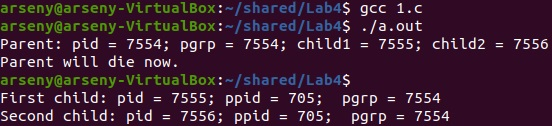
\includegraphics[width=1\linewidth]{inc/img/1.1}}
	\caption{Результат работы программы 1}
	\label{1.1png}
\end{figure}

\begin{figure}[h]
	\center{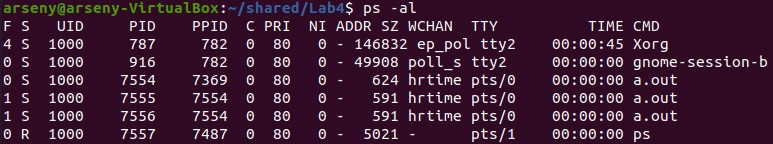
\includegraphics[width=1\linewidth]{inc/img/1.2}}
	\center{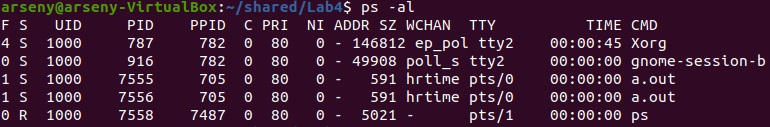
\includegraphics[width=1\linewidth]{inc/img/1.3}}
	\caption{Демонстрация "усыновления"}
	\label{1.2png}
\end{figure}

\newpage
\begin{lstinputlisting}[
	caption={Программа 2},
	label={list2},
	style={c},
	]{../2wait.c}
\end{lstinputlisting}

\begin{figure}[h]
	\center{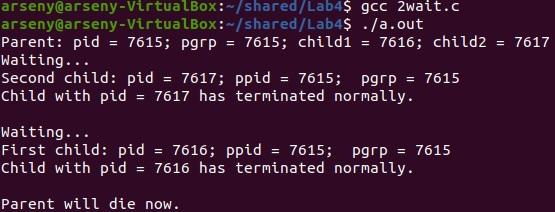
\includegraphics[width=1\linewidth]{inc/img/2.1}}
	\caption{Результат работы программы 2}
	\label{2.1png}
\end{figure}

\newpage
\begin{lstinputlisting}[
	caption={Программа 3},
	label={list3},
	style={c},
	]{../3.c}
\end{lstinputlisting}

\newpage
\begin{lstinputlisting}[
	caption={Программа sort для потомка},
	label={SelectionSortList},
	style={c},
	]{../SelectionSort.c}
\end{lstinputlisting}

\begin{lstinputlisting}[
	caption={Программа print для потомка},
	label={PrintList},
	style={c},
	]{../Print.c}
\end{lstinputlisting}

\begin{figure}[h]
	\center{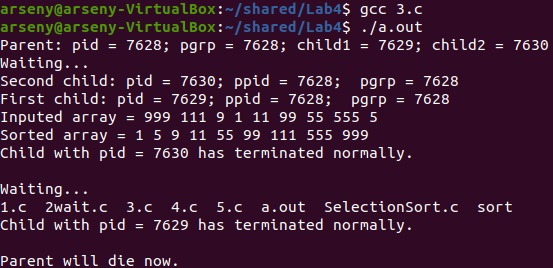
\includegraphics[width=1\linewidth]{inc/img/3.1}}
	\caption{Результат работы программы 3}
	\label{3.1png}
\end{figure}

\newpage
\begin{lstinputlisting}[
	caption={Программа 4},
	label={list4},
	style={c},
	]{../4.c}
\end{lstinputlisting}

\newpage
\begin{figure}[h]
	\center{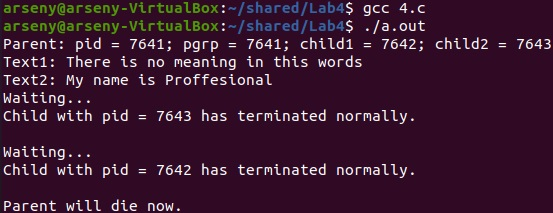
\includegraphics[width=1\linewidth]{inc/img/4.1}}
	\caption{Результат работы программы 4}
	\label{4.1png}
\end{figure}

\newpage
\begin{lstinputlisting}[
	caption={Программа 5},
	label={list5},
	style={c},
	]{../5.c}
\end{lstinputlisting}

\begin{figure}[h]
	\center{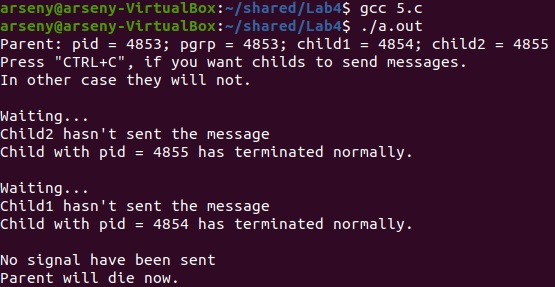
\includegraphics[width=0.9\linewidth]{inc/img/5.1}}
	\center{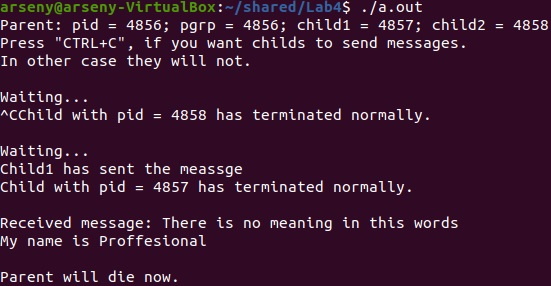
\includegraphics[width=0.9\linewidth]{inc/img/5.2}}
	\caption{Результат работы программы 5}
	\label{5png}
\end{figure}

\newpage
\begin{figure}[h]
	\center{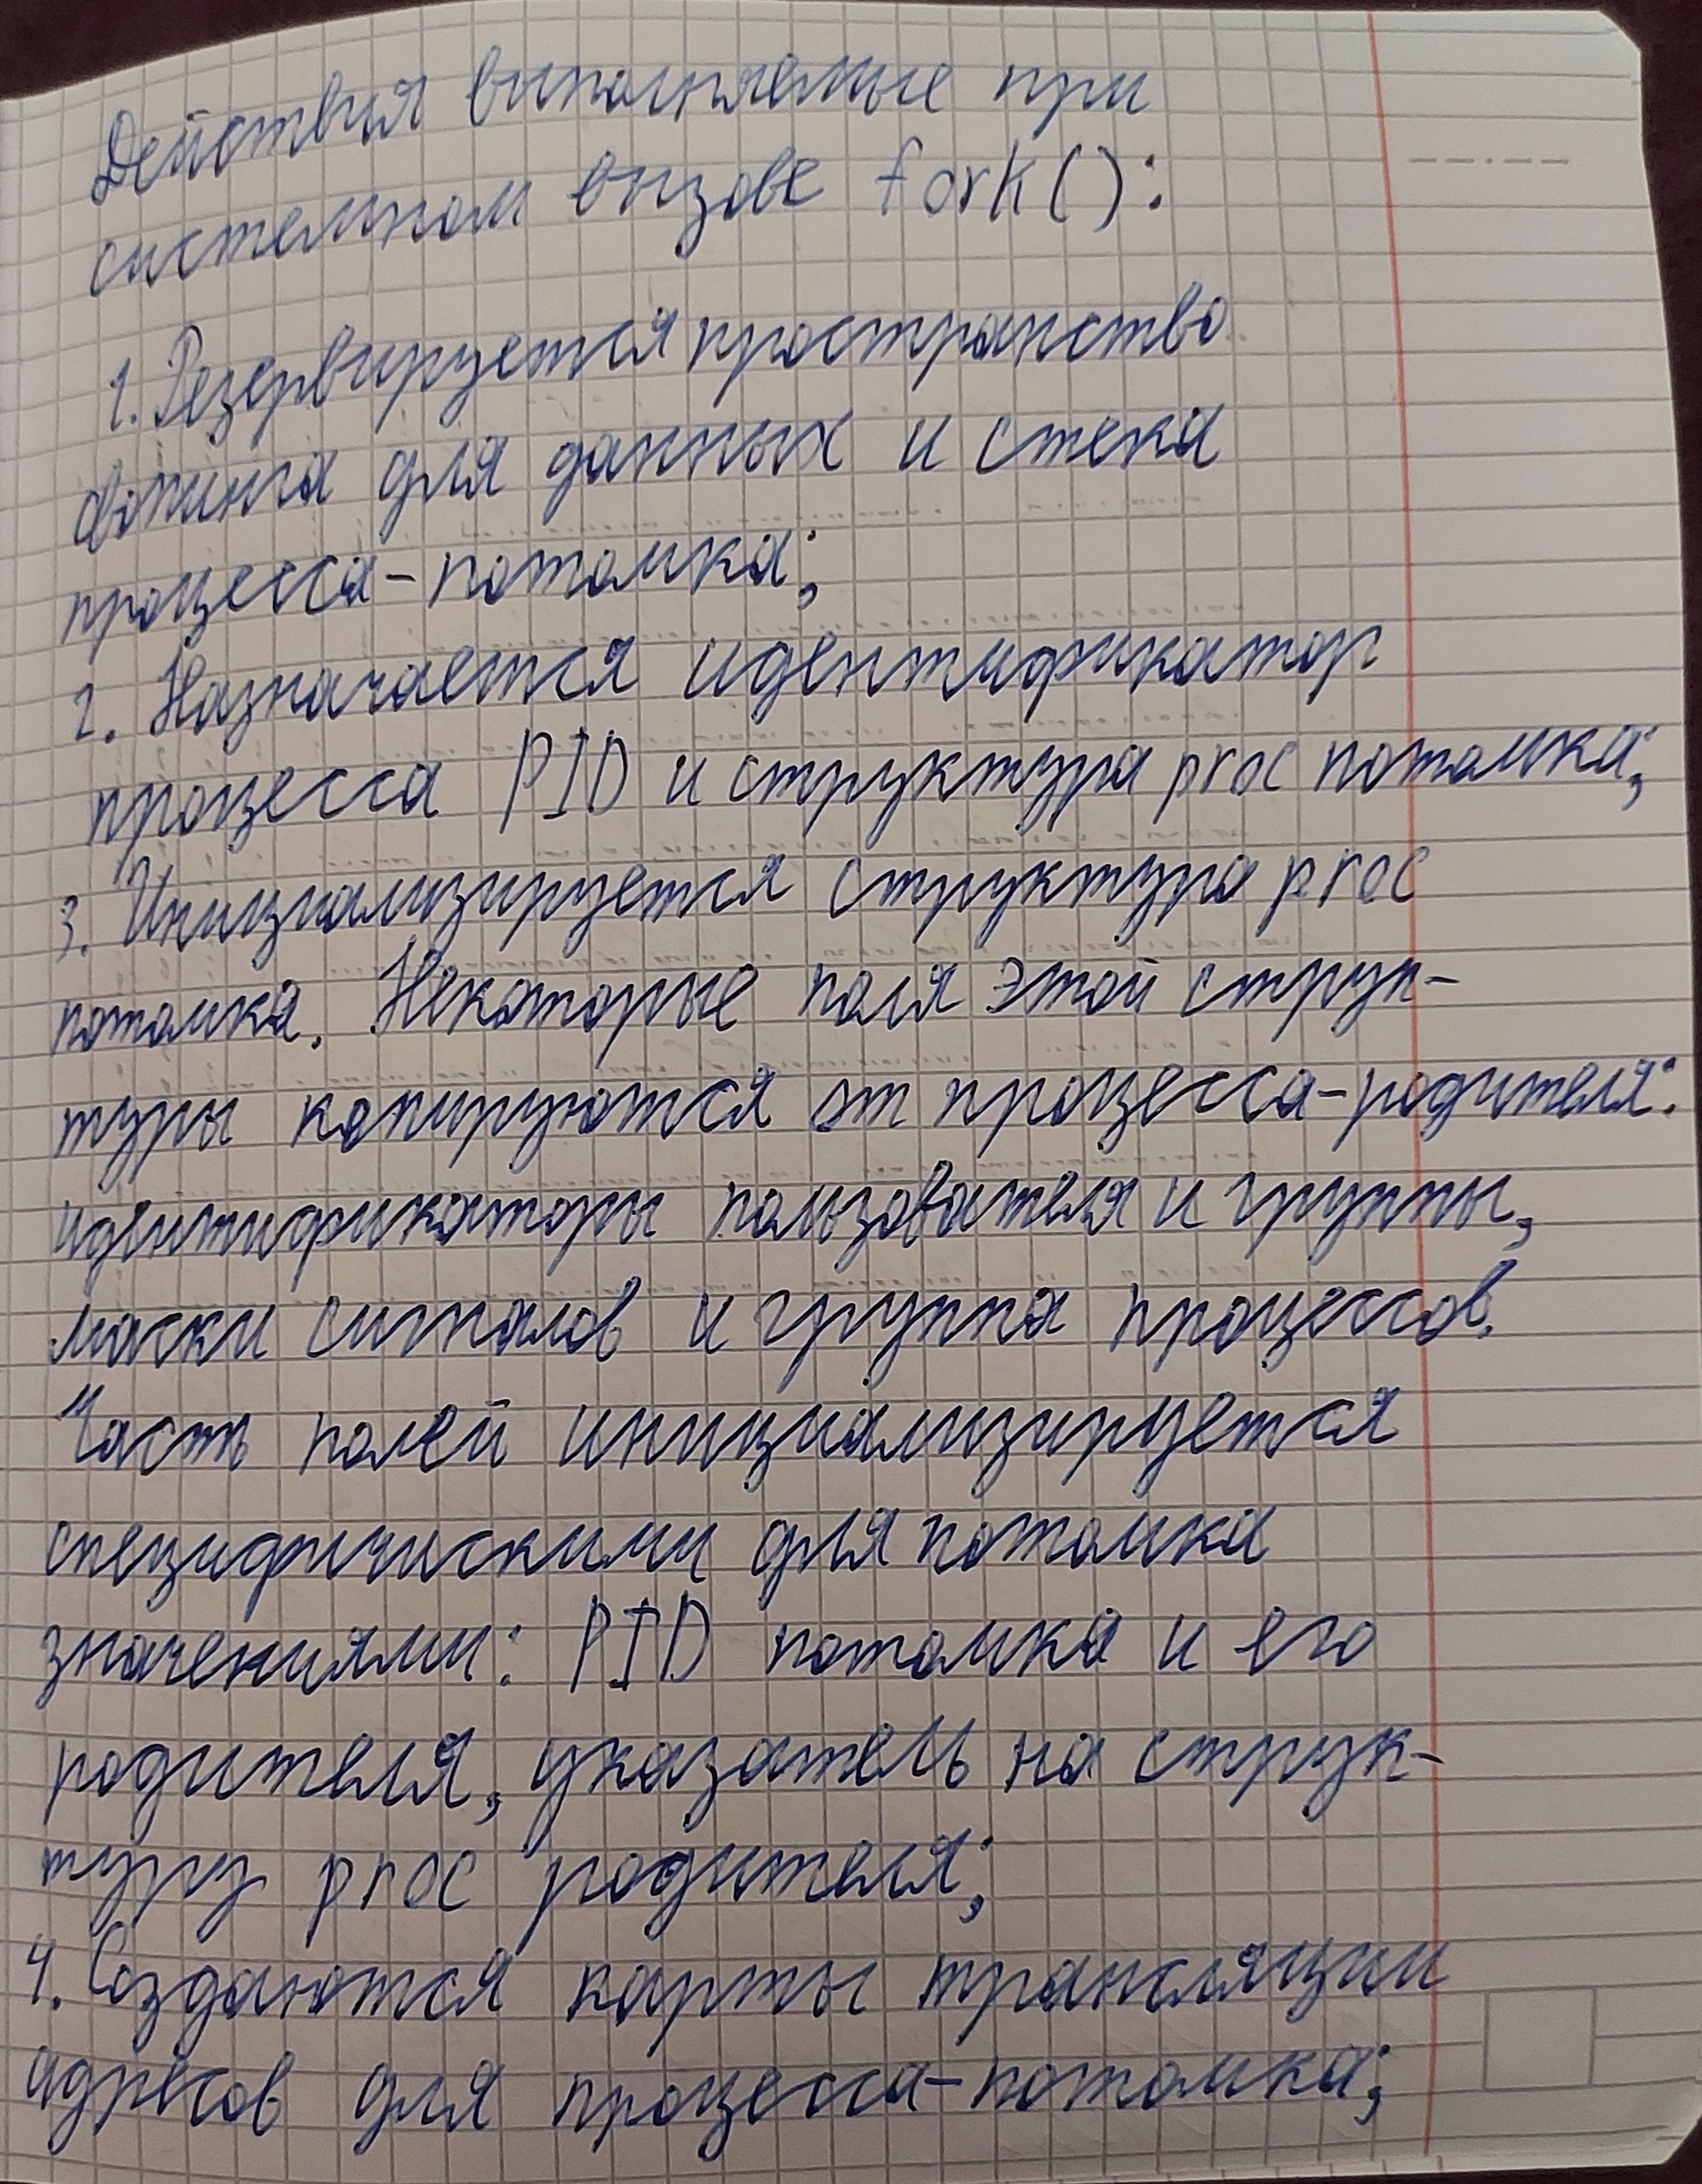
\includegraphics[width=0.9\linewidth]{inc/1}}
	\caption{Действия, выполняемые при системном вызове fork(), стр. 1}
	\label{fork1}
\end{figure}

\begin{figure}[h]
	\center{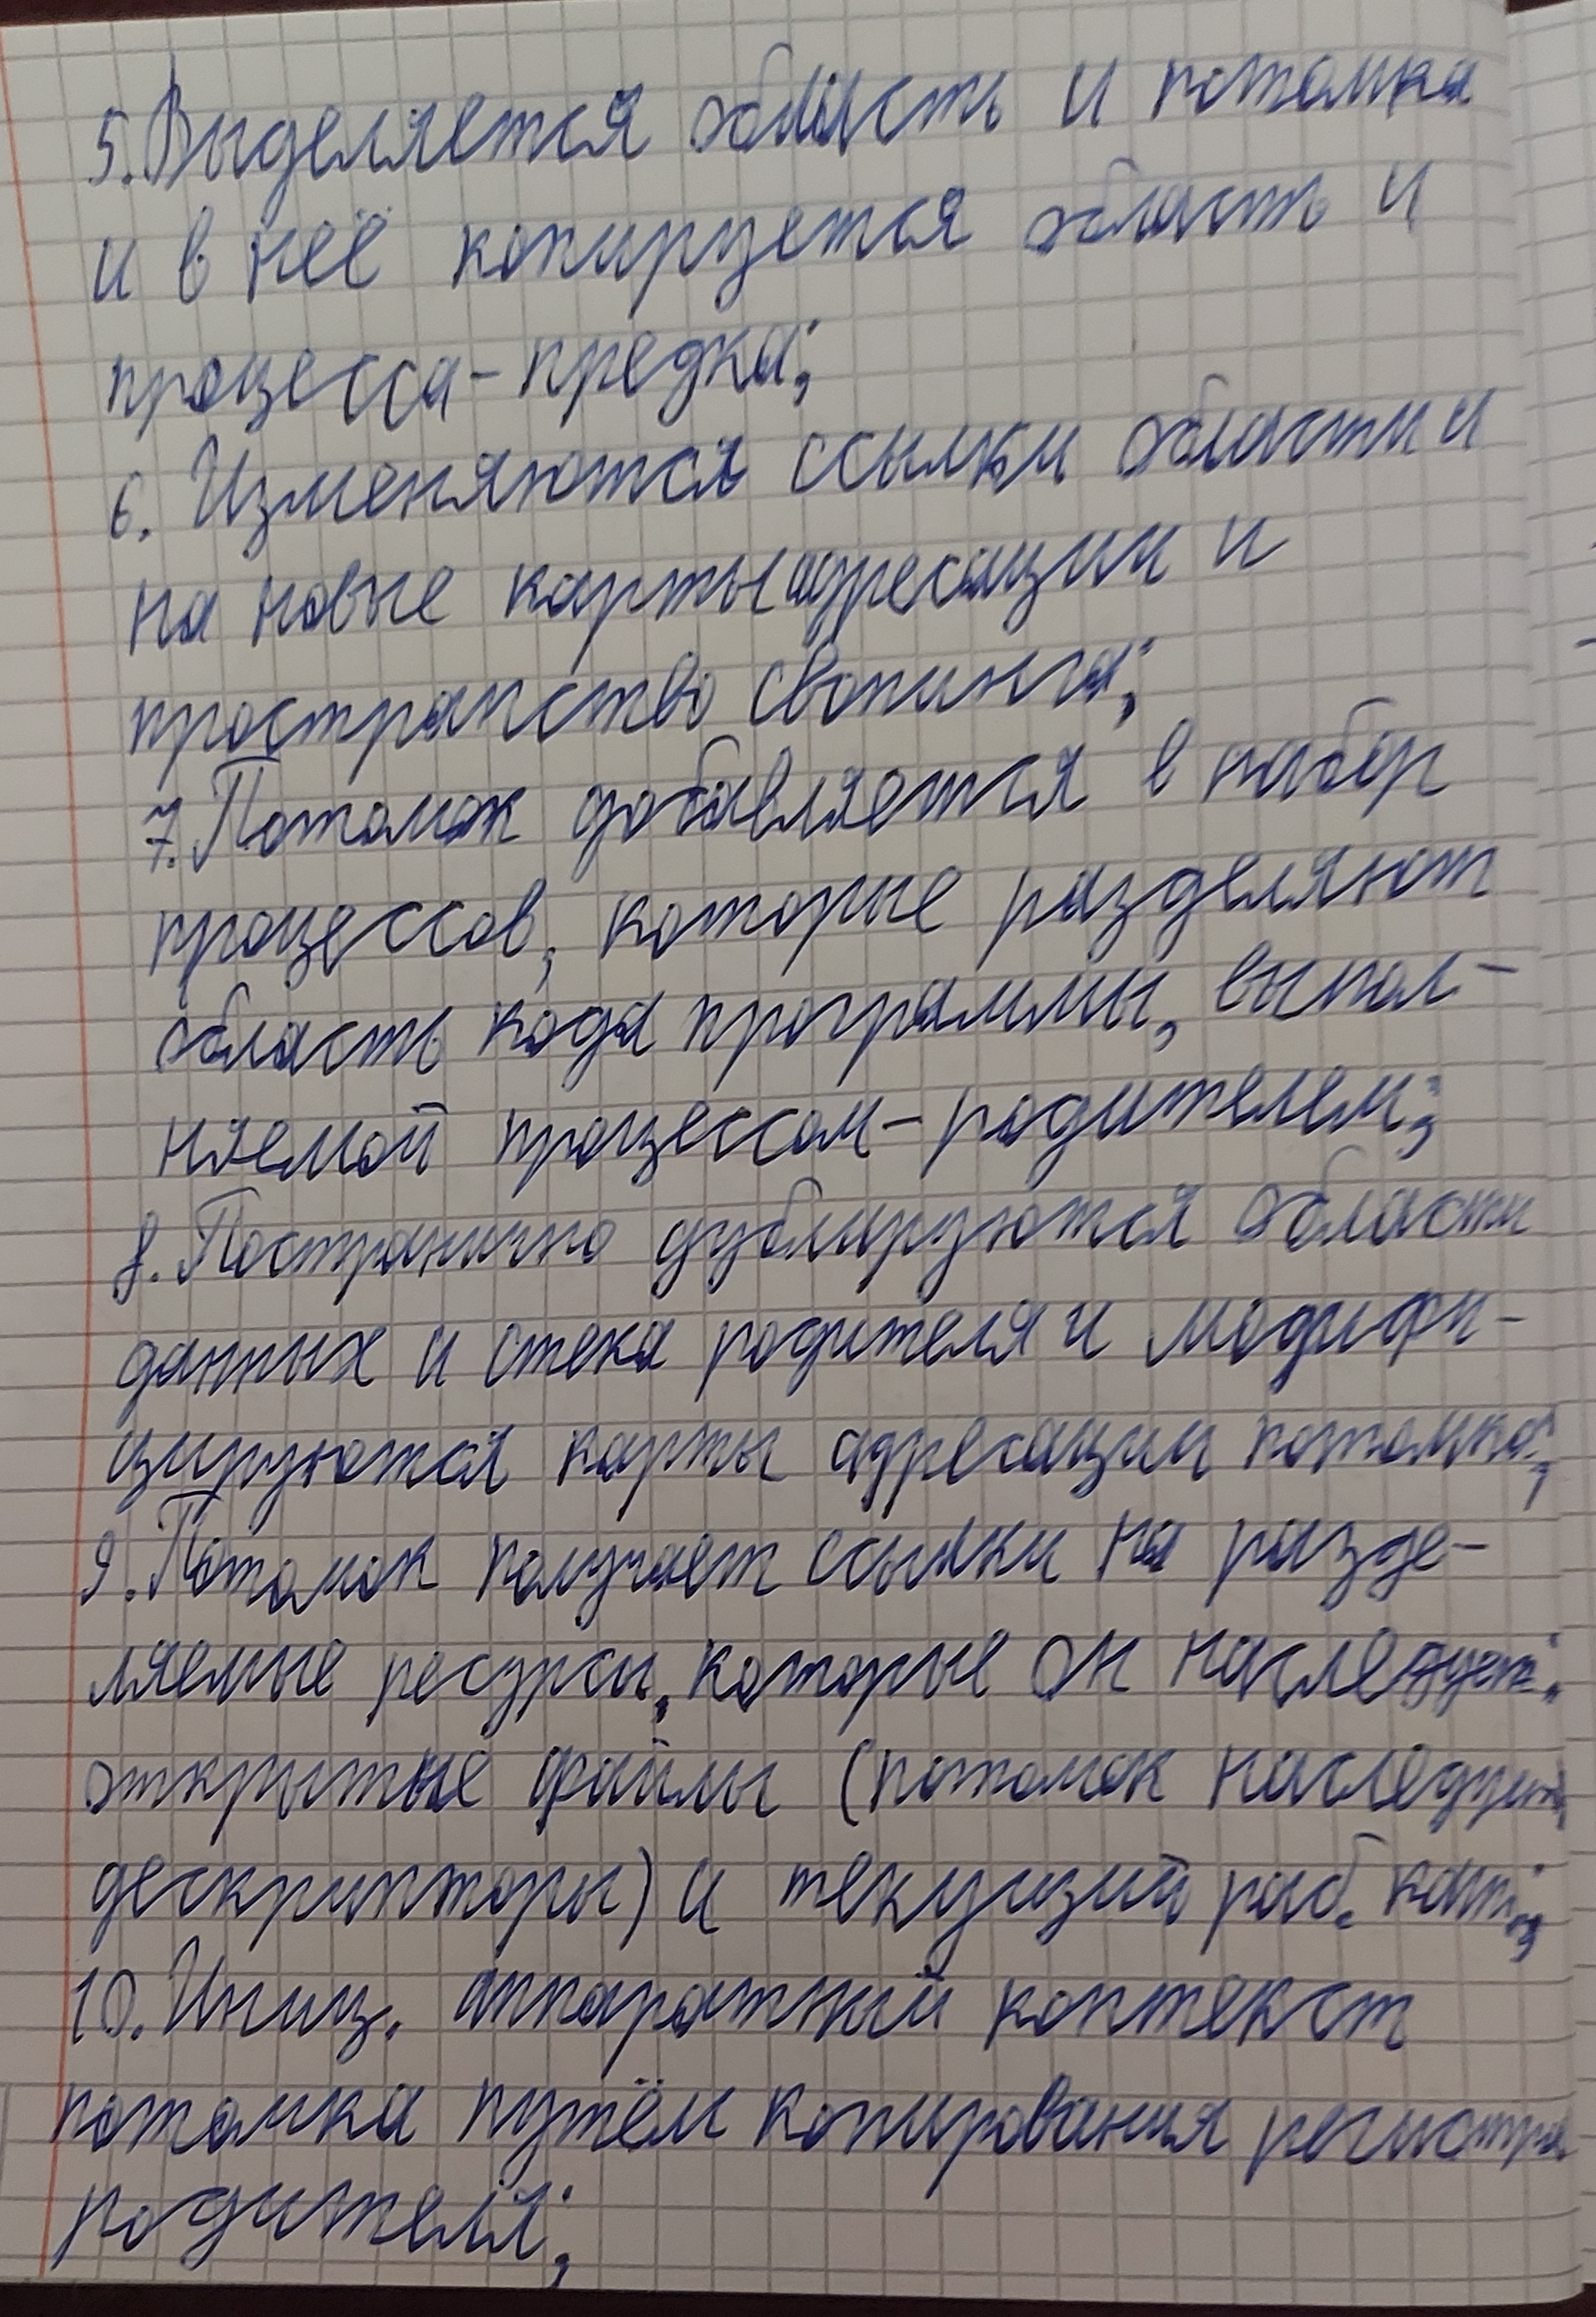
\includegraphics[width=0.9\linewidth]{inc/2}}
	\caption{Действия, выполняемые при системном вызове fork(), стр. 2}
	\label{fork2}
\end{figure}

\begin{figure}[h]
	\center{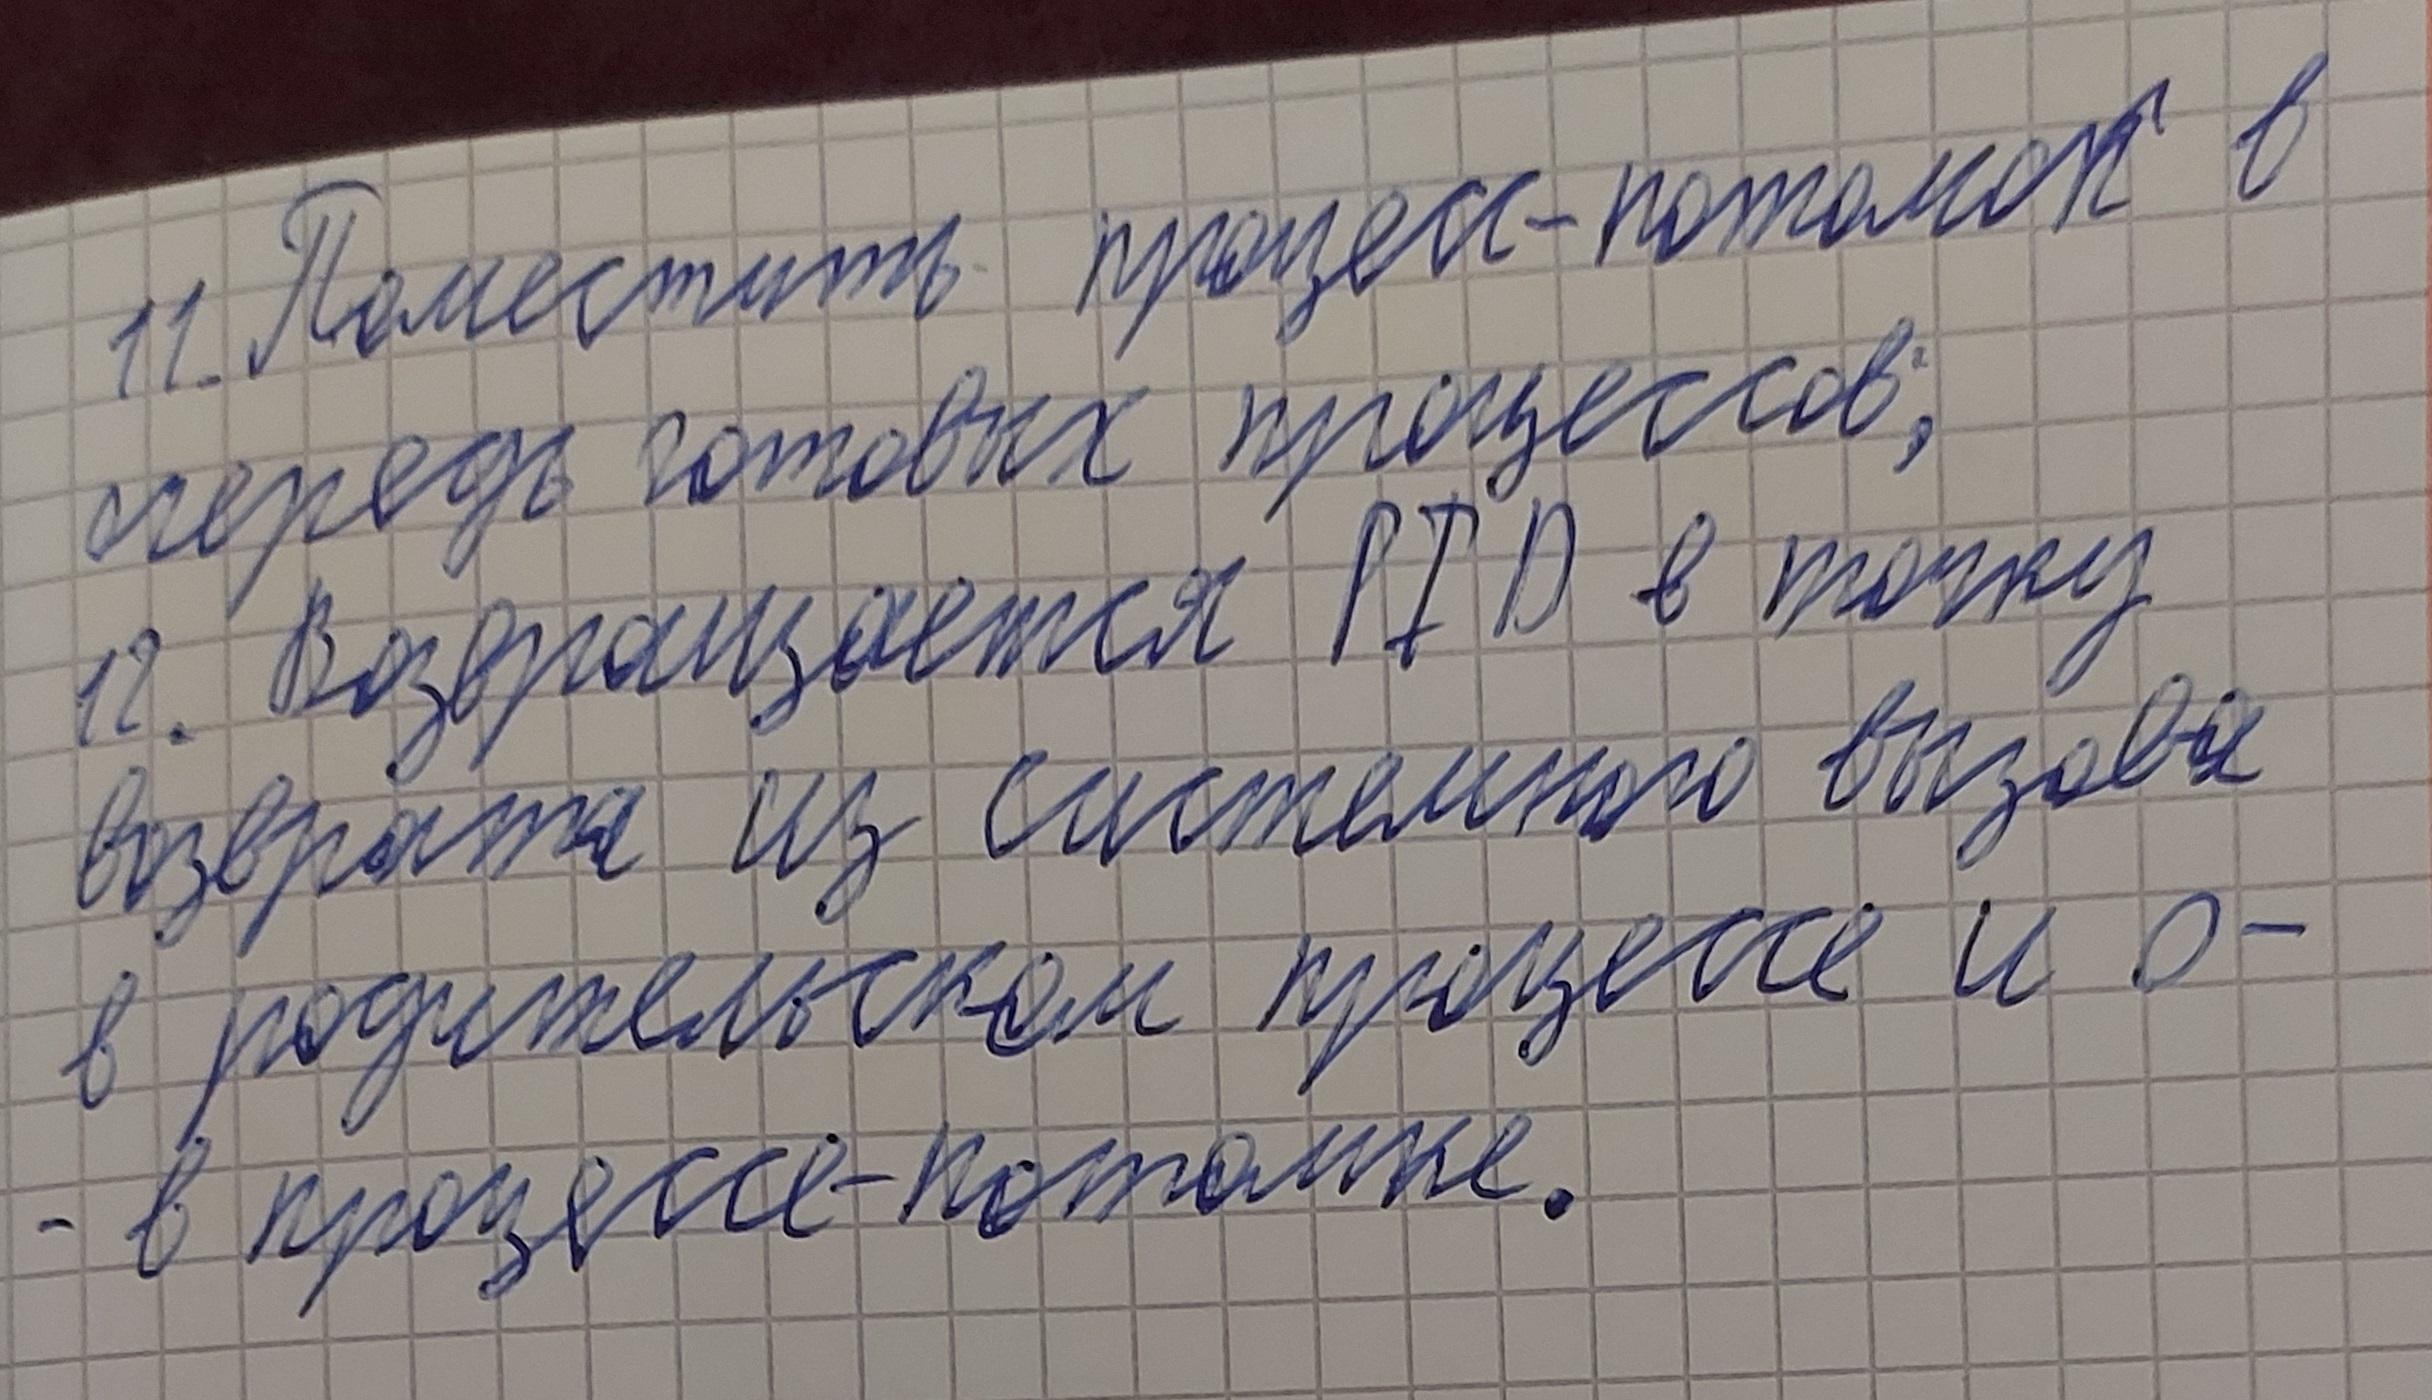
\includegraphics[width=0.9\linewidth]{inc/3}}
	\caption{Действия, выполняемые при системном вызове fork(), стр. 3}
	\label{fork3}
\end{figure}

\newpage
\begin{figure}[h]
	\center{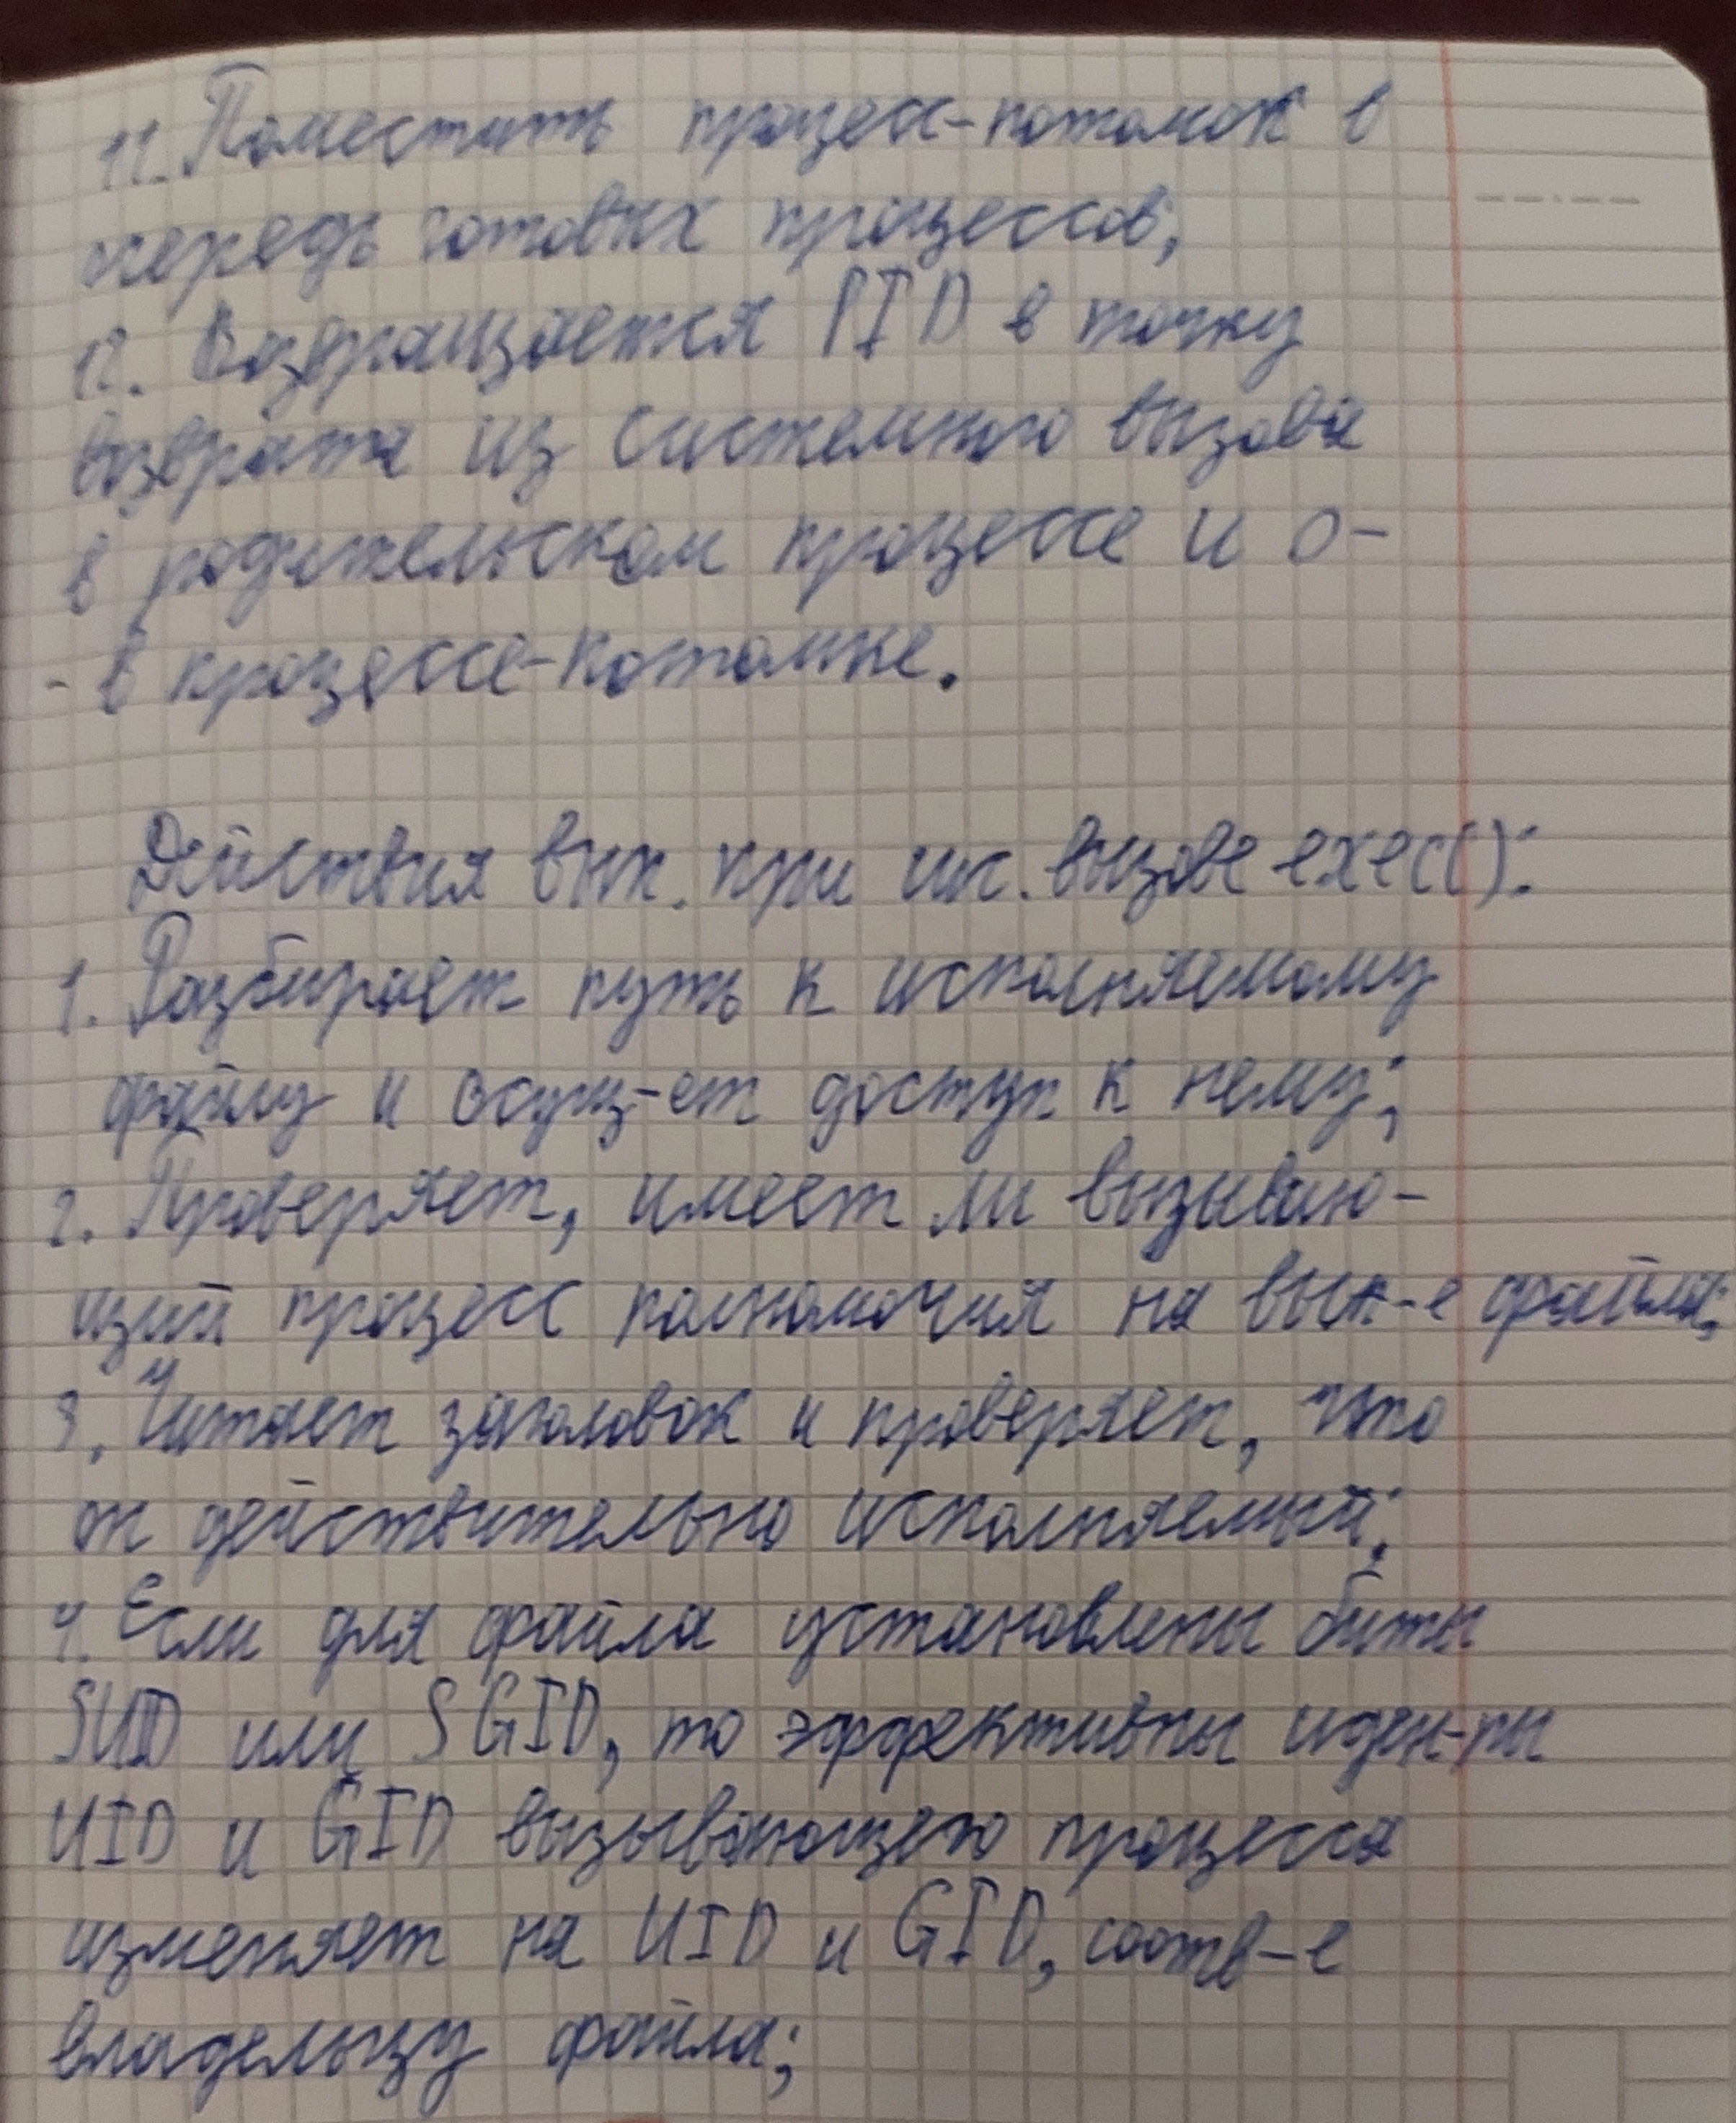
\includegraphics[width=0.9\linewidth]{inc/4}}
	\caption{Действия, выполняемые при системном вызове exec(), стр. 1}
	\label{exec1}
\end{figure}

\begin{figure}[h]
	\center{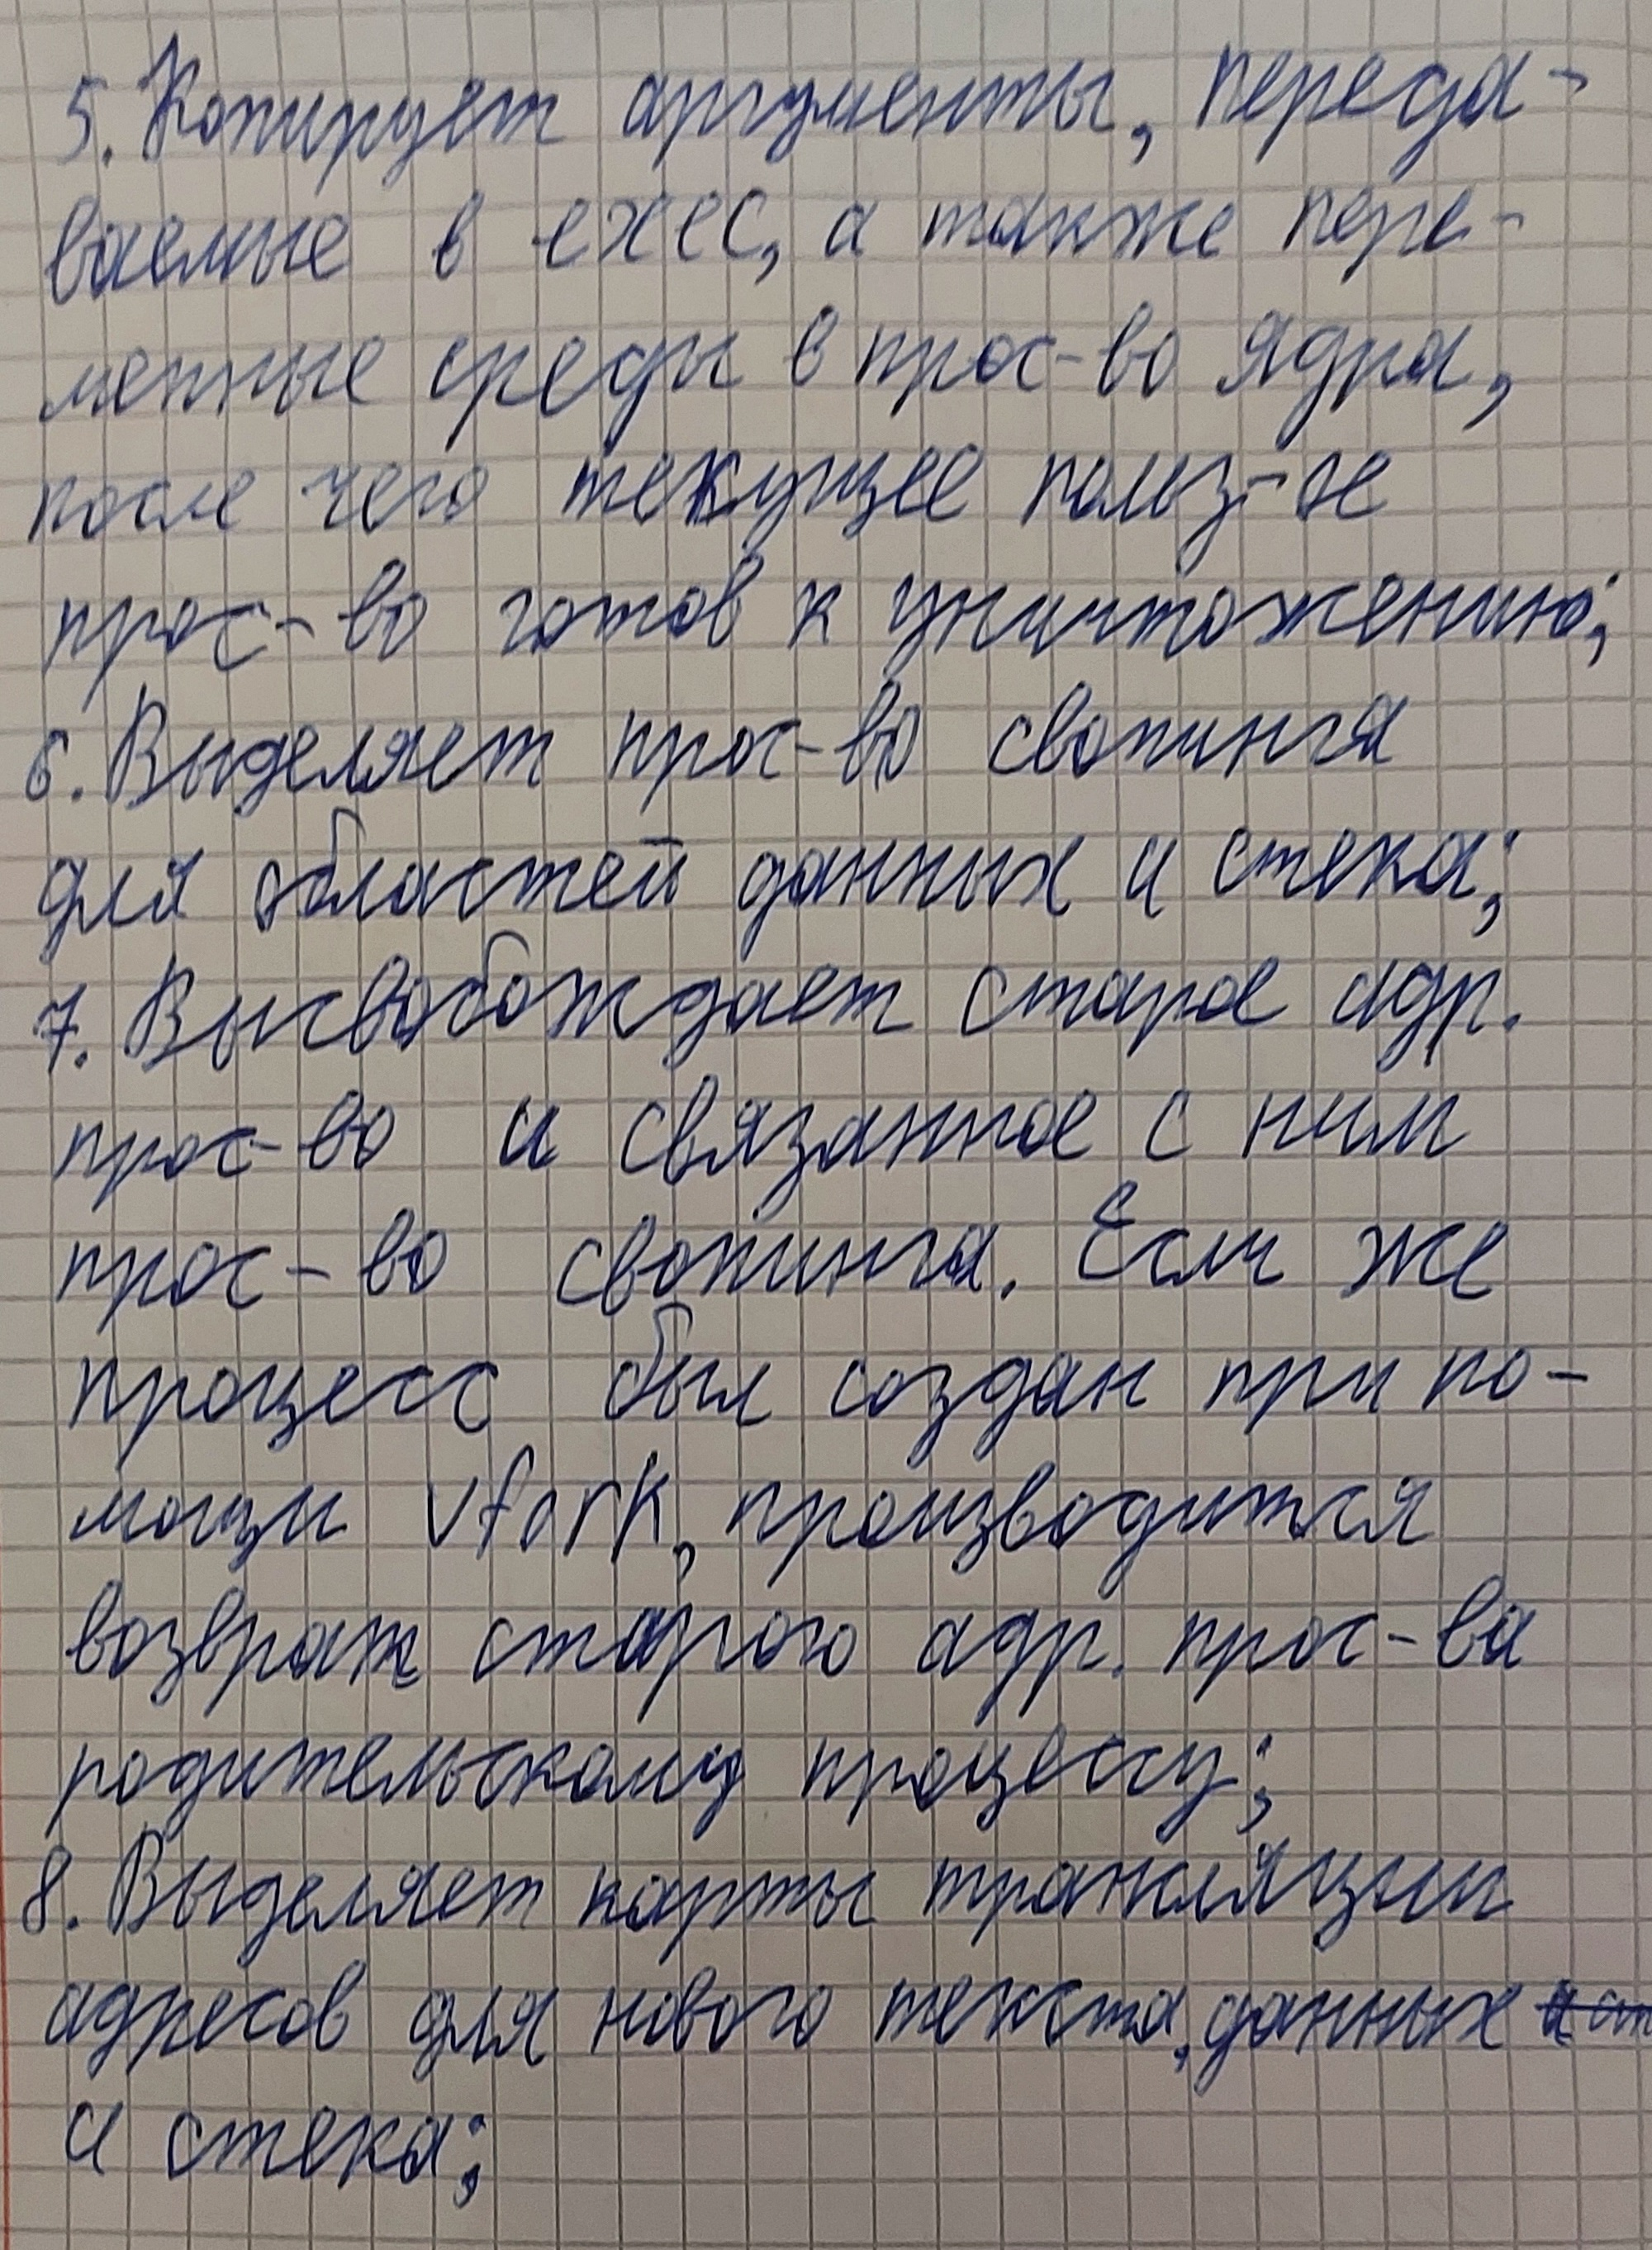
\includegraphics[width=0.9\linewidth]{inc/5}}
	\caption{Действия, выполняемые при системном вызове exec(), стр. 2}
	\label{exeс2}
\end{figure}

\begin{figure}[h]
	\center{
\includegraphics[width=0.9\linewidth]{inc/6}}
	\caption{Действия, выполняемые при системном вызове exec(), стр. 3}
	\label{exec3}
\end{figure}

\begin{figure}[h]
	\center{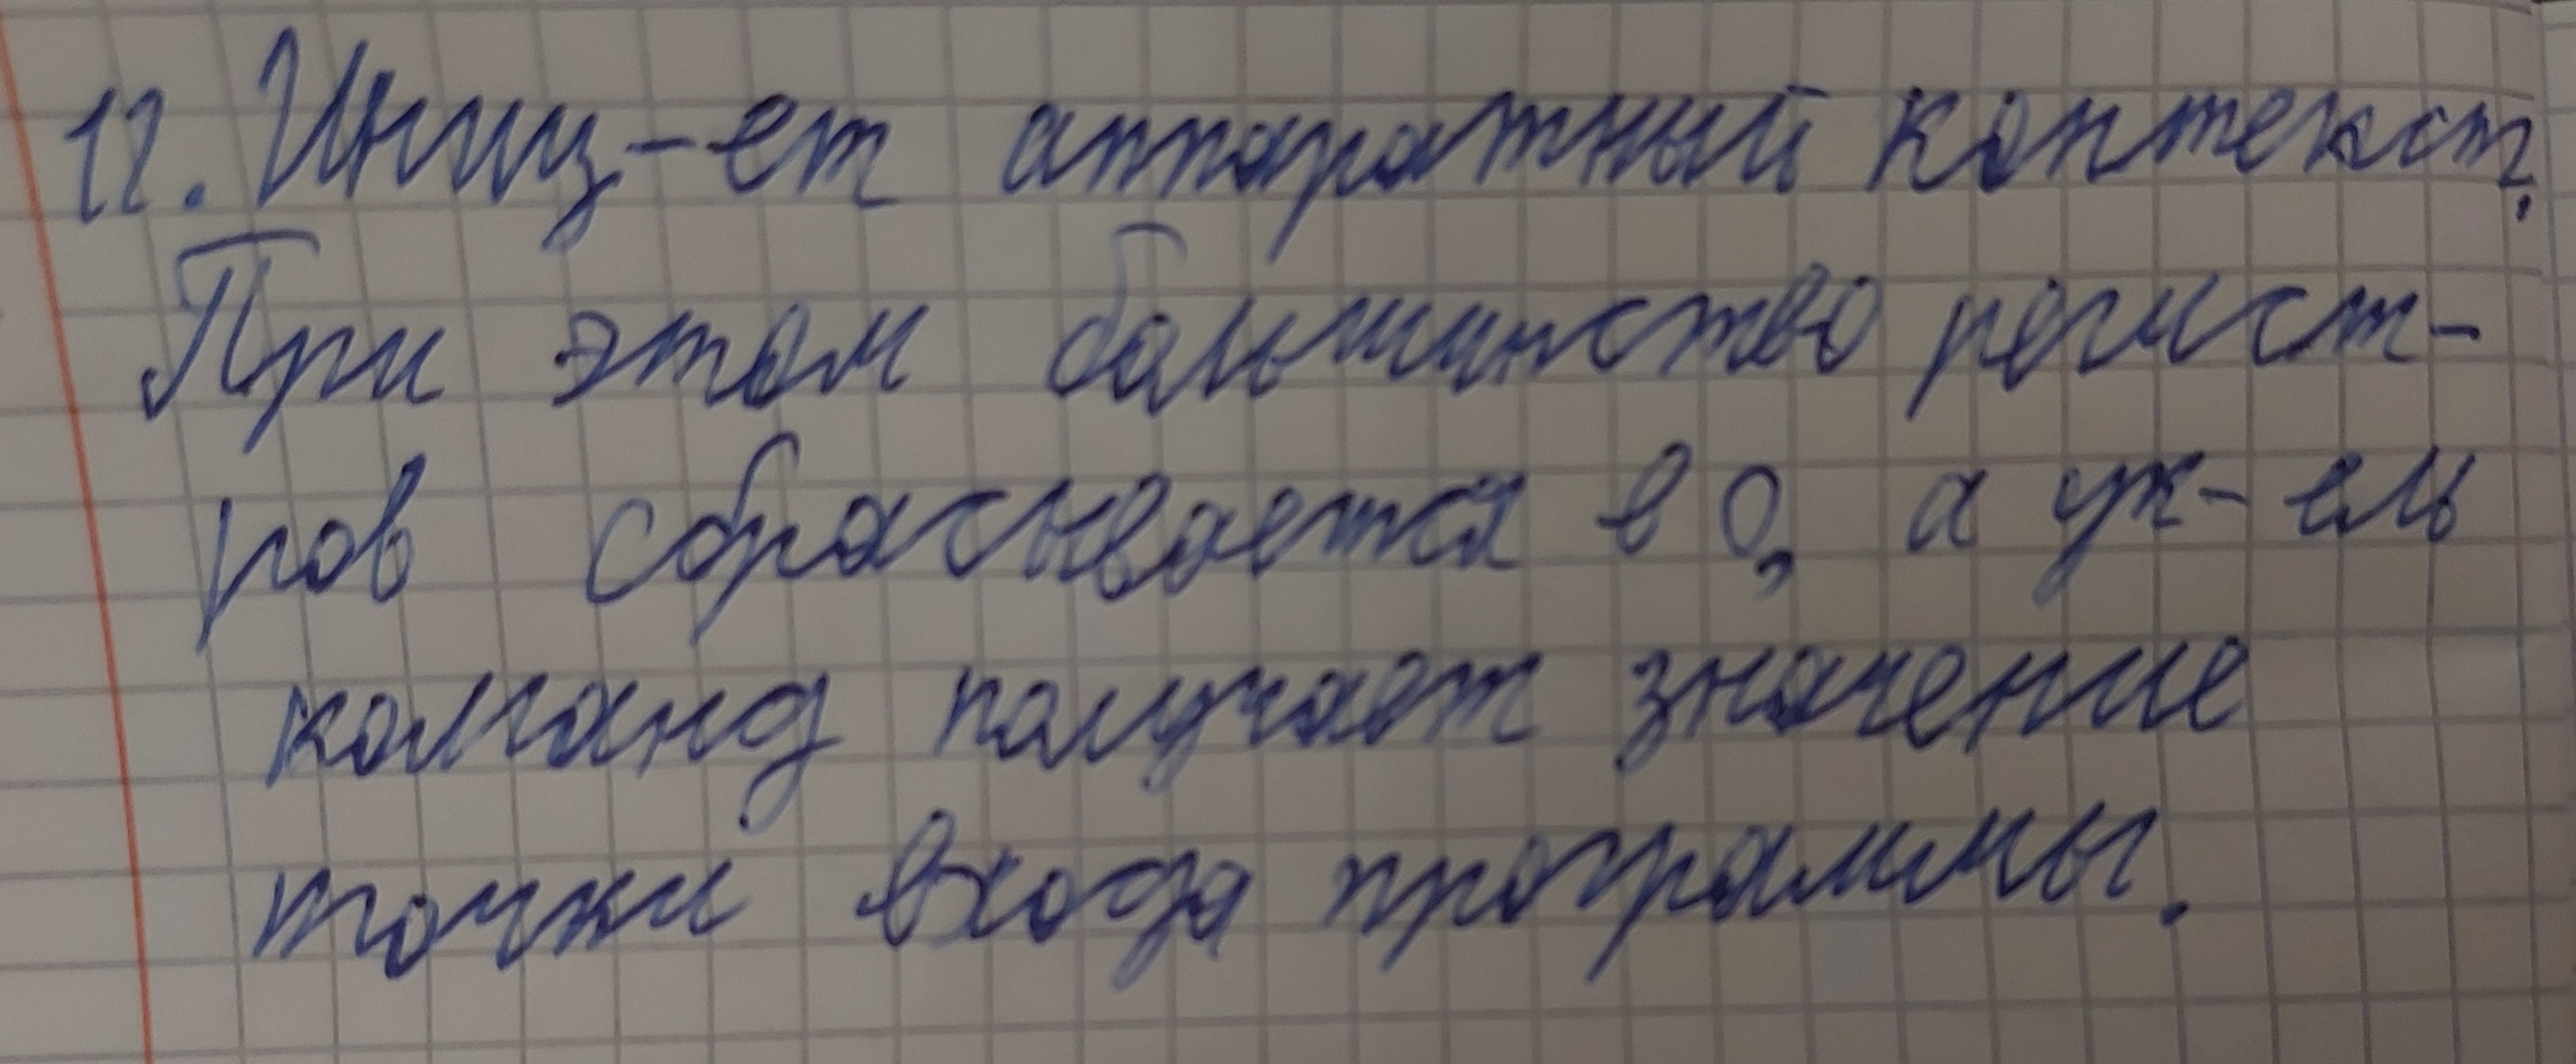
\includegraphics[width=0.9\linewidth]{inc/7}}
	\caption{Действия, выполняемые при системном вызове exec(), стр. 4}
	\label{exec4}
\end{figure}

\end{document}